\documentclass[tikz, crop, border=2]{standalone}

% Schwingende Saite

\usepackage{amsmath}
\usetikzlibrary{math, arrows.meta, decorations.markings, calc, intersections, patterns, 3d, patterns.meta}

\tikzmath{
    \c=cos(115);
    \s=sin(115);
    \r=1.8;
}



\begin{document}
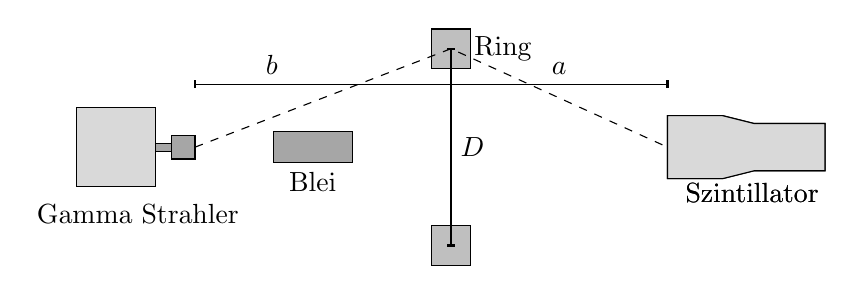
\begin{tikzpicture}[
x={(1 cm, 0 cm)}, y={(0 cm, 1 cm)}, z={(0 cm,-1 cm)},
% #region Picture settings %
ev/.style={-latex, thick},
% #endregion Picture settings %
]


\filldraw[color=black, fill=gray!30] (-1.5,-0.5) node[below=10pt, right=-18pt]{Gamma Strahler} -- (-0.5,-0.5) -- (-0.5,0.5) -- (-1.5,0.5) -- cycle;
\filldraw[color=black, fill=gray!30] (6,-0.4) node[color=black, below=5pt, right=3pt]{Szintillator} -- (6,0.4) -- (6.7,0.4) -- (7.1,0.3) -- (8,0.3) -- (8,-0.3) -- (7.1,-0.3) -- (6.7,-0.4) -- cycle;
\filldraw[color=black, fill=gray!70] (-0.5, -0.05) -- (-0.3, -0.05) -- (-0.3, 0.05) -- (-0.5, 0.05) -- cycle;
\filldraw[color=black, fill=gray!70] (-0.3, -0.15) -- (0, -0.15) -- (0, 0.15) -- (-0.3, 0.15) -- cycle;
\filldraw[color=black, fill=gray!50] (3,1) node[color=black, above=7,  right=12pt]{Ring} -- (3,1.5) -- (3.5,1.5) -- (3.5,1) -- cycle;
\filldraw[color=black, fill=gray!50] (3,-1) -- (3,-1.5) -- (3.5,-1.5) -- (3.5,-1) -- cycle;
\filldraw[color=black, fill=gray!30] (6,-0.4) node[color=black, below=5pt, right=3pt]{Szintillator} -- (6,0.4) -- (6.7,0.4) -- (7.1,0.3) -- (8,0.3) -- (8,-0.3) -- (7.1,-0.3) -- (6.7,-0.4) -- cycle;
\filldraw[color=black, fill=gray!70] (1,-0.2) node[color=black, below=7pt, right=2pt]{Blei} -- (1,0.2) -- (2,0.2) -- (2,-0.2) -- cycle;


\draw (0,0.8) -- (3.25,0.8) node[pos=0.3, above]{$b$};
\draw[thick] (0,0.75) -- (0,0.85);
\draw[thick] (3.25,0.75) -- (3.25,0.85);

\draw (3.25,0.8) -- (6,0.8) node[pos=0.5, above]{$a$};
\draw[thick] (6,0.75) -- (6,0.85);
\draw[thick] (3.25,0.75) -- (3.25,0.85);

\draw (3.25, -1.25) -- (3.25, 1.25) node[pos=0.5, right]{$D$};
\draw[thick] (3.2,1.25) -- (3.3,1.25);
\draw[thick] (3.2,-1.25) -- (3.3,-1.25);

\draw[dashed] (0,0) -- (3.25,1.25) -- (6, 0);

\end{tikzpicture}
\end{document}